\clearpage
\section{Results}
\label{sec:results}

The numerical example in this section is based on the initial capacities of the four major electricity producers in Germany from figure \ref{fig:capacities}. We estimate the potential investment behaviour for a three-period horizon. Longer time horizons are possible, but lead to a larger amount of computational time and do not add much more economic insight. We consider rea time horizon of nine years, where investment decision have to be taken in $t=0,3,6$. Market equilibria for the production decisions have to be obtained in each node, also including the set of terminal nodes $\mathcal{S}$ in $t=9$.  The uncertainty is modeled with the calibrated scenario tree in figure \ref{fig:intercept}.

\subsection{Scenario generation}

We use the proposed procedure in from section \ref{sec:scenario-generation} with an estimate of $6\%$ for the growth of the market volume, which corresponds to the CAGR for 2002-2006 obtained from \cite{Datamonitor2007}. The calibrated scenario tree for the highest price segment from table \ref{tab:marketsegments} can be seen in figure \ref{fig:intercept}.

\begin{figure}[htb]
  \centering
\caption{Demand function intercept $\alpha_n^m$ with growth rate $\rho_e=0.06$}
  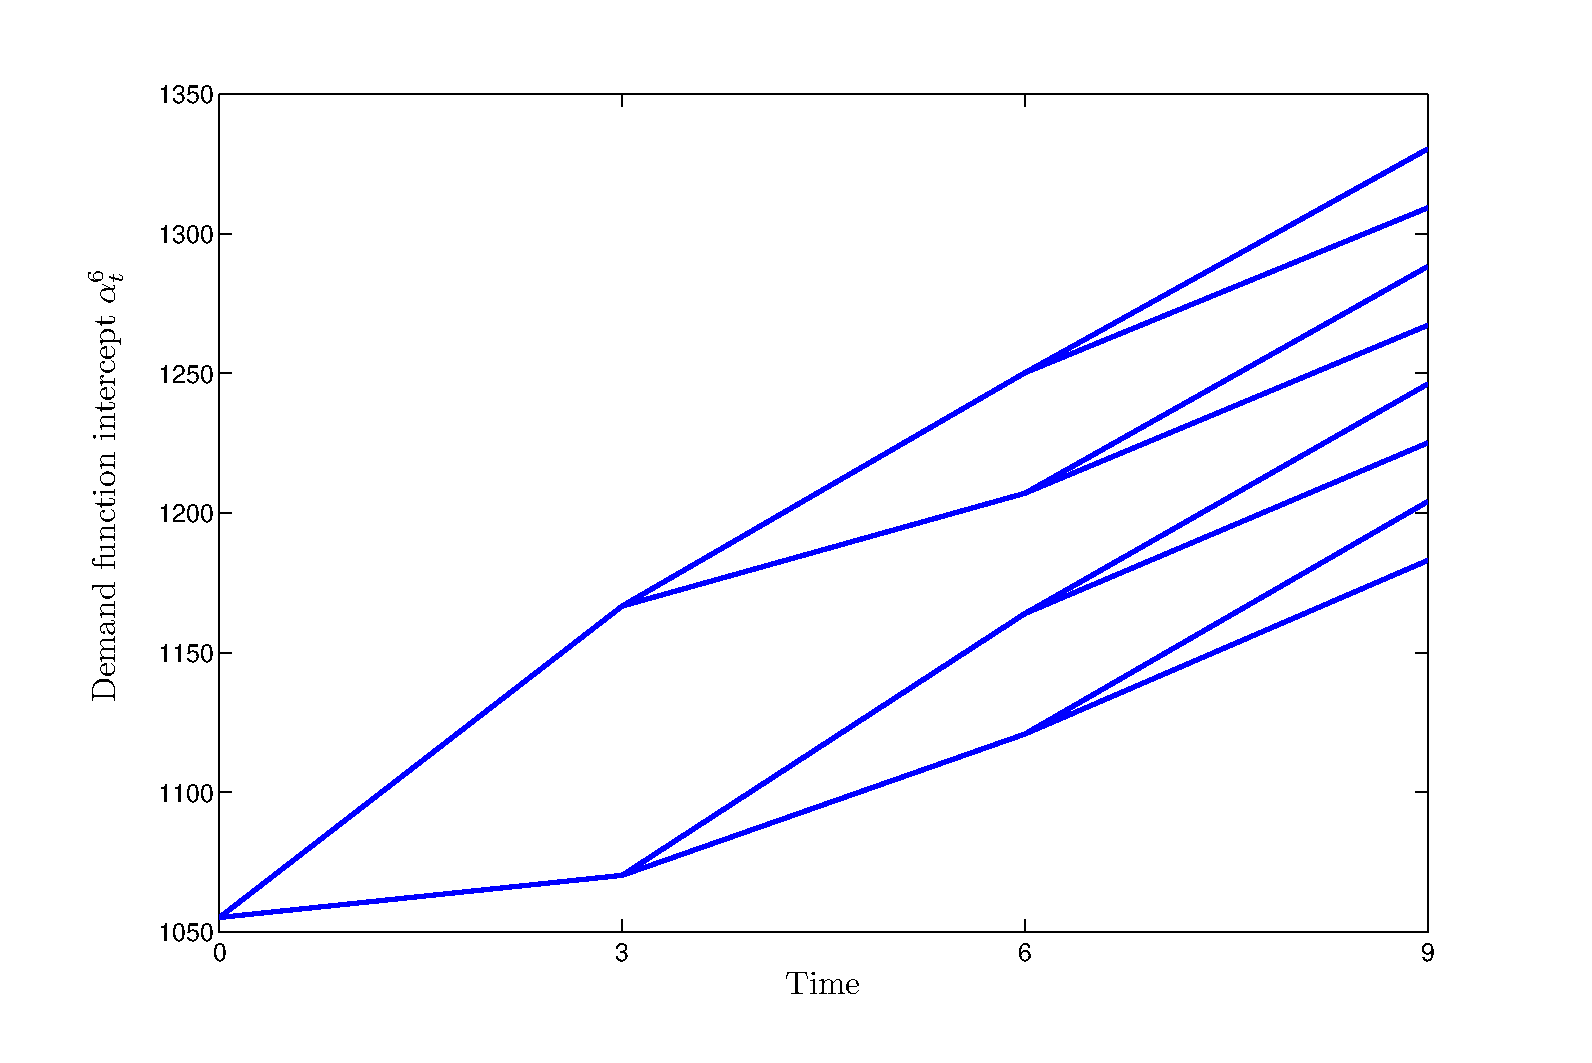
\includegraphics[width=0.75\textwidth]{intercept}
  \label{fig:intercept}
\end{figure}


\subsection{Solution of the MCP}

We have implemented the mixed complementarity problem (MCP) in \eqref{eq:kkt_first}-\eqref{eq:kkt_last} in GAMS (General Algebraic Modelling System) and solved with with the PATH solver \citep[see][]{Ferris2000}.

Table \ref{tab:}

\begin{table}[htb]
  \centering
  \caption{Investment}
  \vspace{0.3cm}
  \begin{tabular}{rrr}
    
  \end{tabular}
\end{table}


%%% Local Variables: 
%%% mode: latex
%%% TeX-master: "gencapinvest"
%%% End: 
